\section*{Results}

In order to demonstrate our method, we run it on D-NeRF's~\cite{pumarola2020dnerf} synthetic dataset which contains 8 different rendered scenes with simple movement. These scenes have ground truth camera positions, viewing directions and timestamps. They capture physically plausible movement, without large discontinuities or jumps between frames.

We also demonstrate our method on a closed-room dataset, the Gibson dataset rendered for NeRFlow~\cite{du2021nerflow} using the iGibson environment~\cite{xu2019DISN}. This contains a single moving TurtleRobot from many similar views, similar to LLFF datasets.

We also note that we compare our method to our own implementation of NR-NeRF, to isolate the difference between our approach and using just an MLP. We make some modifications, by passing time explicitly rather than a latent vector, not varying regularization over epochs, and not requiring that at time $t=0$ we have no deformation in the rays.

\subsection*{Qualitative Results}

The difference between our work and NR-NeRF can be observed in the difference of flow between scenes. It can be observed from Fig.~\ref{fig:qual_cmp} that our method captures coherent movement for objects, whereas for NR-NeRF movement may not be in the same direction, and we define coherence loosely as having similar movement within nearby space. For example, on the ball (top right), a significant portion does not appear to be moving. In addition, for the Lego scene (bottom left), our method isolates the loader on the tractor, whereas NR-NeRF cannot.

The difference between the two is also more clearly seen in videos of reconstruction. Spline-NeRF visibly has the effect of ``tweening'' between views, slowing into stops, while NR-NeRF appears less smooth.

\subsection*{Quantitative Results}

The qualitative comparison of our method to NR-NeRF is shown in Tab.~\ref{tab:dnerf_cmp}. Spline-NeRF is able to perform on par or with minimal degraded performance with our implementation of NR-NeRF on D-NeRF's synthetic dataset. This is likely because NR-NeRF does not impose constraints on the velocity or acceleration of movement, whereas Spline-NeRF is forced to create a smooth interpolation, which is more difficult. To be more precise, Spline-NeRF \textit{must} learn a continuous function, which is strictly more constrained than the set of functions that an MLP can learn, as the MLP can reproduce the observed views at each time, and implicit smooth between views. In practice NR-NeRF learns fairly smooth movement, but quantitatively looks different from our methods' movement, due to differences in velocity and acceleration. Bezier splines enforce that movement is fluid and can better reproduce in-between frames, trading off reproduction quality for smoothness. We expect that in longer sequences and data with larger gaps Spline-NeRF would benefit from this constraint.

\subsection*{Gibson Dataset}

We also include a more realistic dataset from NeRFlow~\cite{du2021nerflow}, the Gibson dataset, rendered from the iGibson environment~\cite{xu2019DISN}. Our method has median PSNR $24.537$ dB and $0.886$ SSIM, and NR-NeRF has median PSNR $24.591$ dB and $0.887$ SSIM. Instead of the mean, we use the median since there are test frames which contain an object close to the camera which is rarely seen in the training set, thus there are some frames with extremely low quality on both methods. Fig.~\ref{fig:gib_cmp} highlights the differences, notably, our method produces coherent movement, despite having lower quantitative metrics, and this can be seen in NR-NeRF's artifacts and the motion flow fields.

\begin{table*}[t]
    \centering
    \begin{tabular}{|c| c|c | c|c | c|c | c|c |}
    \hline
    \textbf{PSNR$^\uparrow$ $|$ MS-SSIM$^\uparrow$} & \multicolumn{2}{c|}{Bouncing Balls} & \multicolumn{2}{c|}{Hellwarrior$^\dagger$} & \multicolumn{2}{c|}{Hook} & \multicolumn{2}{c|}{Jumping Jacks} \\
    \hline
    NR-NeRF & \textbf{27.573} & \textbf{0.984}
           & 33.314 & 0.968
           & 27.954 & 0.978
           & 28.476 & 0.985 \\
    \hline
    Spline-NeRF & 26.418 & 0.979
               & 33.504 & 0.968
               & 28.104 & 0.979
               & 28.424 & 0.986 \\
    \hline
    & \multicolumn{2}{c|}{Lego} & \multicolumn{2}{c|}{Mutant} & \multicolumn{2}{c|}{Standup} & \multicolumn{2}{c|}{T-Rex} \\
    \hline
    NR-NeRF & 23.663 & 0.946
           & 30.382 & 0.989
           & 31.624 & 0.989
           & 26.649 & 0.985 \\
    \hline
    Spline-NeRF & 23.656 & 0.943
               & 31.183 & 0.992
               & 31.349 & 0.990
               & 26.056 & 0.982 \\
    \hline
    \end{tabular}
    \vspace{2pt}
    \caption{
        \label{tab:dnerf_cmp}
        \textbf{Comparison of mean PSNR and MS-SSIM for Spline-NeRF and NR-NeRF.} Bolded values are those that are significantly greater than the other.
        Bezier splines are able to recover movement with near equal accuracy in dynamic scenes as compared to NR-NeRF~\cite{tretschk2021nonrigid}. Due to the forced prior of continuous movement, we learn a smooth interpolation through each frame. We randomly samples all frames from the start of training. Here, we parametrize Spline-NeRF with 5 control points. \newline
        $^\dagger$We had difficulty consistently reproducing results on this dataset. This is mostly because it is extremely dark: it is difficult to distinguish the black background from the object.
    }
    \vspace{-6mm}
\end{table*}

\begin{figure*}
    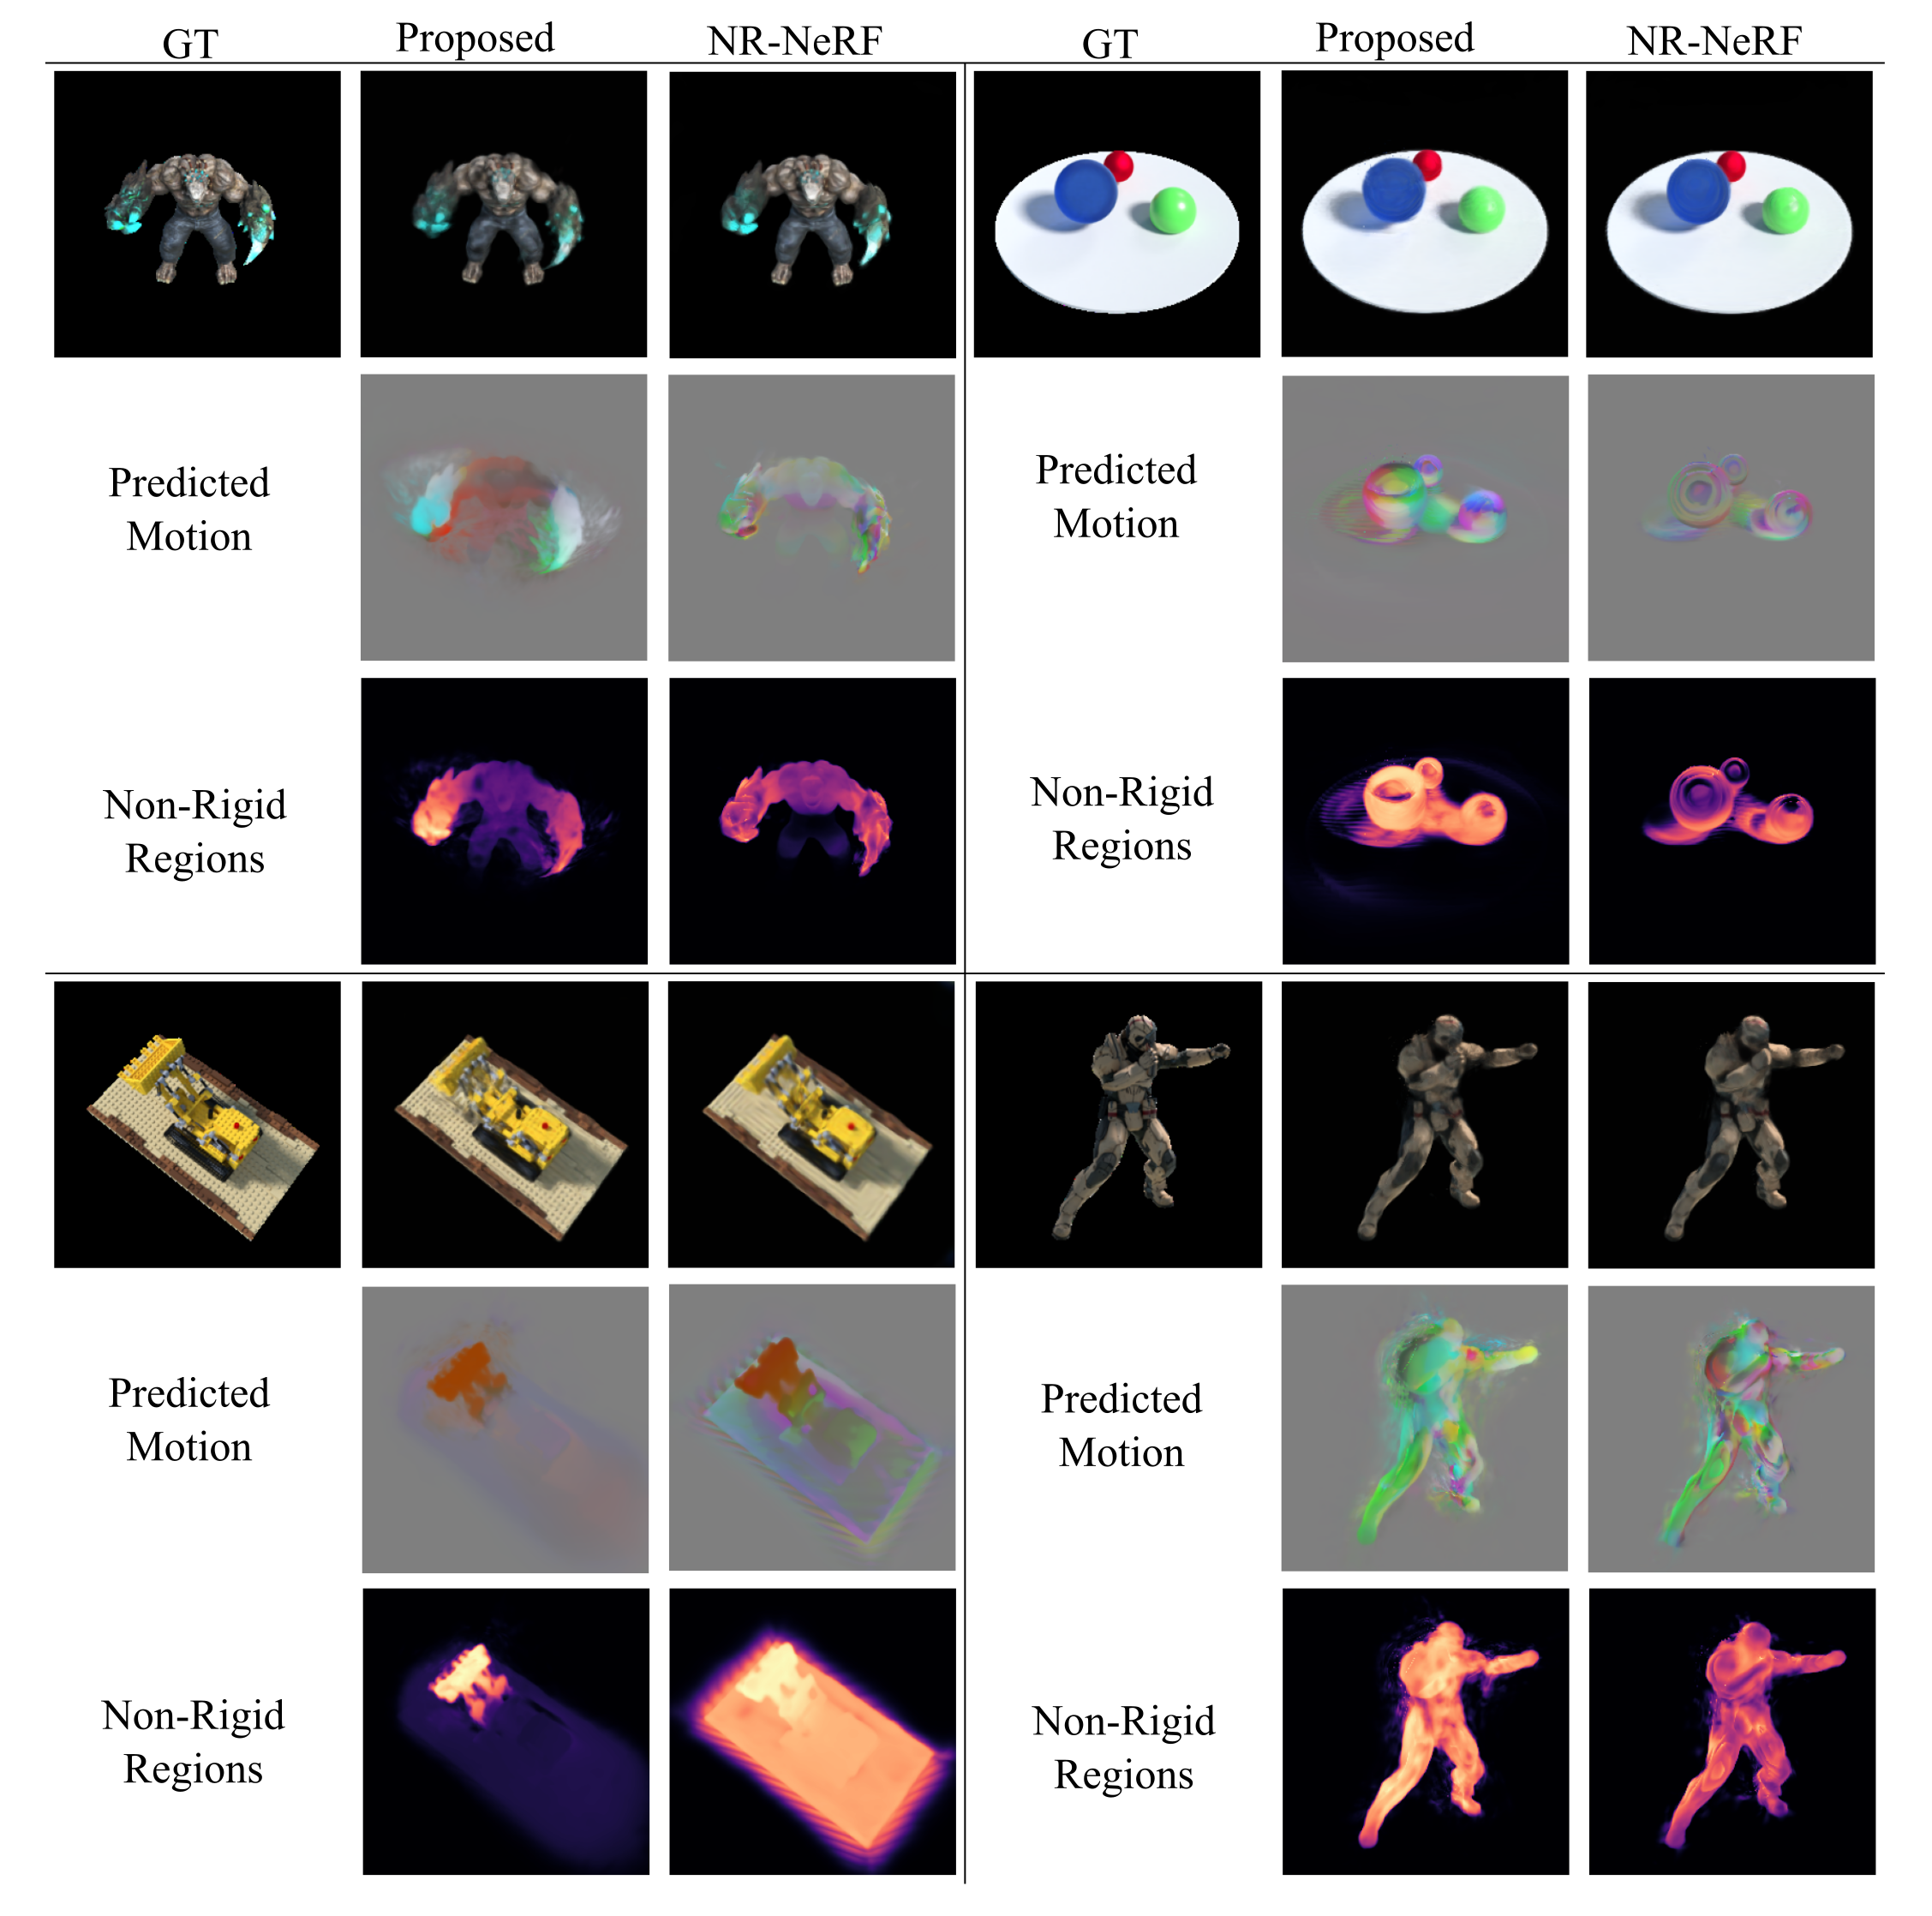
\includegraphics[width=\textwidth]{compare}
    \caption{
        \label{fig:qual_cmp}
        \textbf{Visual comparison of Spline-NeRF to NR-NeRF.}
        Results comparing movement in our implementation of NR-NeRF~\cite{tretschk2021nonrigid} versus the proposed approach for using Bezier splines for modelling movement. The direction of motion is shown by color, distance is shown by intensity, and gray is 0 motion. Non-rigid regions are visualized as brighter. There is substantial difference in the predicted motion, and this can be seen in the Mutant and Hook scenes (top left, bottom right respectively), where NR-NeRF predicts very noisy 3D flow, but our approach is coherent, where coherence is loosely defined as being similar to nearby points. There is also a large difference in rigidity, where the spline has highly coherent non-rigid regions. This is especially noticeable in the Lego scene (bottom left), where NR-NeRF makes the entire model non-rigid, but adding a spline isolates the loader on the tractor to be non-rigid. We expect this is because splines are forced to have similar scale for movement, and the rigidity is less needed to compensate for error or differences in scale. For an MLP, it may predict different scales of motion for nearby points, but rigidity can compensate for this since it doesn't strictly learn 0 or 1.
        \
        The quality of the output is similar. In some portions, NR-NeRF captures higher quality output, such as in the shadows of the balls, or in the crispness of the Mutant's blue claws. On the other hand, the spline more accurately captures the knobs and shadows of the knobs on the Lego scene.
    }
\end{figure*}

\begin{figure*}[!ht]
    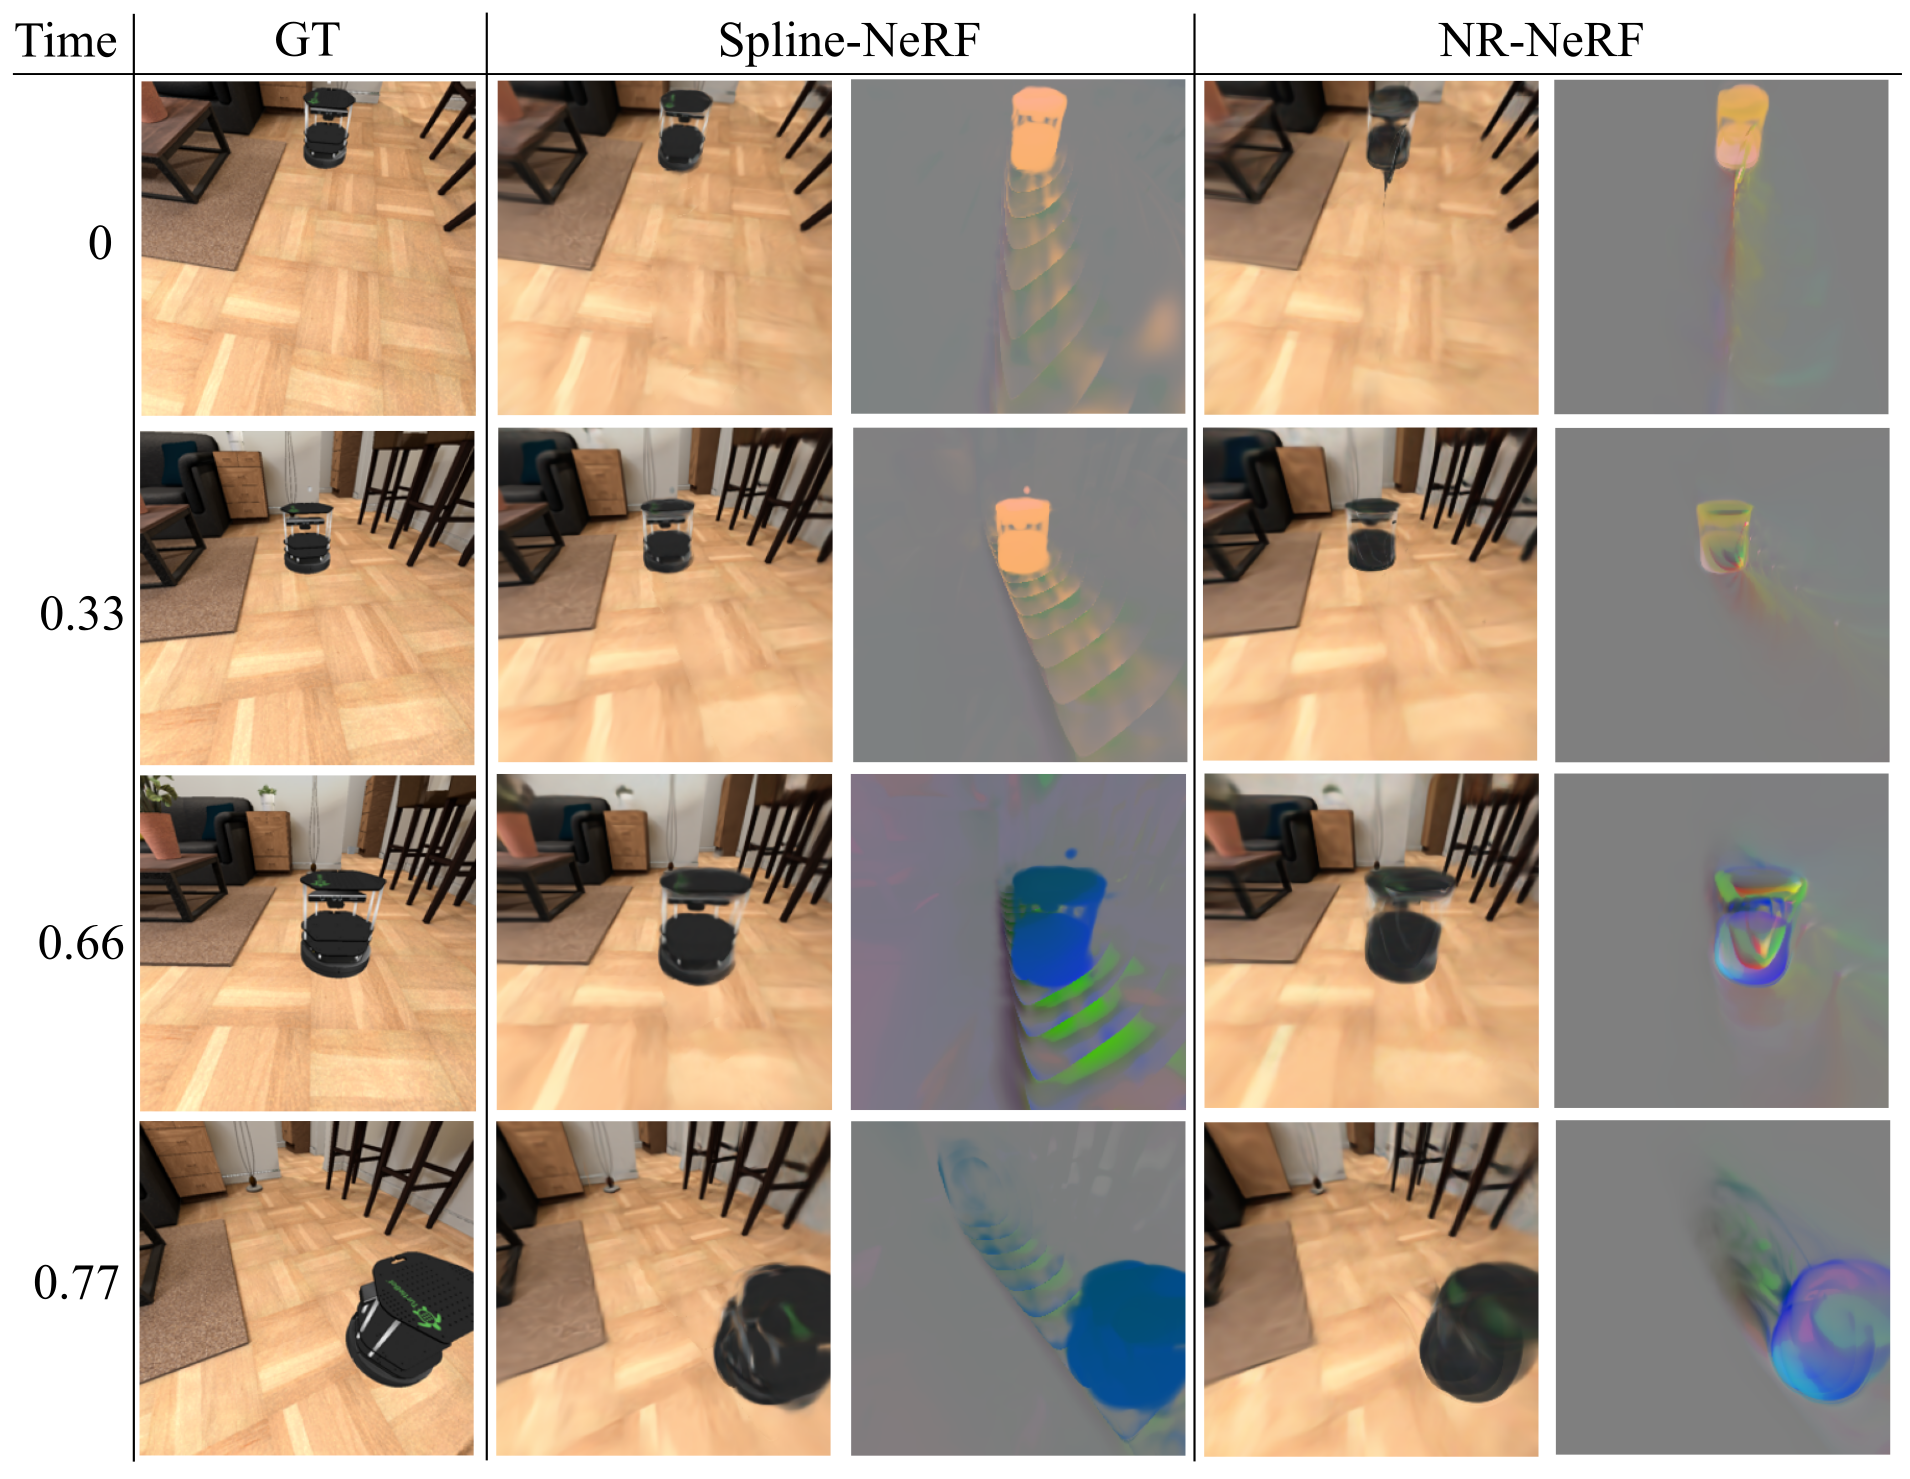
\includegraphics[width=\textwidth]{gibson_cmp}
    \caption{
        \label{fig:gib_cmp}
        \textbf{Visual comparison of Spline-NeRF to NR-NeRF on Gibson Dataset.} Our method produces coherent movement as compared to NR-NeRF, and is also visually more coherent, despite having a lower PSNR and MS-SSIM. It can be easily seen that the TurtleBot in NR-NeRF has artifacts, and does not move as a whole unit, whereas Spline-NeRF moves the whole robot uniformly. We do not include samples around $t=1$, since both our approach and NR-NeRF produce low-quality reconstructions around those times.
    }
    \vspace{-6mm}
\end{figure*}
